\chapter{Results}

The main goal of this analysis was to quantify key metrics of the performance of LGAD sensors. In particular, we analysed the collected charge, the time resolution and the efficiency at the temperature of \qty{-30}{\degreeCelsius}. We compared the results between unirradiated and differently irradiated sensors to test whether the requirements at start and end of life were satisfied. The sensors were also examined angled to the beam direction (between \qty{0}{\degree} and \qty{14}{\degree}), as, when HGTD will be operational, it will cover pseudorapidities between $2.4$ and $4$, corresponding to an incident angle between \qty{2}{\degree} and \qty{10}{\degree}.

Additionally, some other properties and effects that arose during the analysis were also investigated. Such as, signal coming from neighbouring pads, noise coming from outside the gain layer of the pads, interference between adjacent pads, and properties of the region lying between two adjacent pads. Certain anomalies were also successfully explained, and the root cause was found in the incorrect range of voltages set on an oscilloscope, which caused pulses to be "clipped" below a specific threshold. Moreover, due to a temporary malfunction of the cooling box, one particular batch of data showed neatly the influence of temperature on the properties of LGADs.



\section{Main Results}

\begin{figure}[h!tbp]
    \centering
    \includegraphics[width=.9\linewidth]{Images/Results/Irradiated/IME_voltage_charge_.png}
    \captionsetup{width=\captionwidth}
    \caption{Maybe this should include ALL sensors}
    \label{fig:irradiated_IME_voltage_charge}
\end{figure}


\begin{figure}[h!tbp]
    \centering
    \includegraphics[width=.9\linewidth]{Images/Results/Irradiated/IME_voltage_time_resolution_.png}
    \captionsetup{width=\captionwidth}
    \caption{}
    \label{fig:irradiated_IME_voltage_time_res}
\end{figure}

The most important properties of the sensors are:

\begin{itemize}
    \item Collected change: the most probable value (MPV) of the Landau*Gaussian convolution (\ref{sec:methods_collected_charge}).
    \item Time resolution: the spread of the Gaussian distribution of the Time of Arrivals (\ref{sec:methods_time_resolution}).
    \item Efficiency: the number of hits picke up by sensors over the total (\ref{sec:methods_efficiency}).
\end{itemize}

Overall all sensors behaved as expected: their collected charge increased with higher bias voltage and decreased with higher radiation dose (fluence).

\subsection{Irradiated}

\subsubsection{IME}

The sensors in the IME group were then further split depending on versions and types, to enable more meaningful comparisons between devices with similar characteristics.

%%% IMEv3-W12, 0 and 
\begin{figure}[h!tbp]
    \centering
    \subfloat[Voltage vs Charge.]{
        \includegraphics[width=.49\linewidth]{Images/Results/Irradiated/IMEv3-W12_voltage_charge_irradiated.png}
        \label{fig:IMEv3-W12_voltage_charge}}
    \hfill
    \subfloat[Voltage vs Time resolution]{
        \includegraphics[width=.47\linewidth]{Images/Results/Irradiated/IMEv3-W12_voltage_time_resolution_irradiated.png}
        \label{fig:IMEv3-W12_voltage_time_res}}
    \vfill
    \subfloat[Voltage vs Efficiency]{
        \includegraphics[width=.47\linewidth]{Images/Results/Irradiated/IMEv3-W12_voltage_efficiency_irradiated.png}
        \label{fig:IMEv3-W12_voltage_efficiency}}
    \captionsetup{width=\captionwidth}
    \caption{IMEv3-W12. The non irradiated sensors (both the 2x2 array and the 1x3 array) had sufficiently high collected charge at all tested bias voltages, while the time resolution was just short of the \qty{35}{\pico\second} target in the case of the 2x2 array, although this is likely to be solved with higher applied voltage. The lack of data for higher voltages was due to erronous batches. It should be noted that the two pads of the 1x3 array had significant and consistent discrepancies in charge and time resolution, presumably due to manufacturing differences. The sensors at \qty{1.5e15}{\neutroneq} had very good performance overall and reached the target time resolution of the beginning of operations at $\simeq60\%$ of the total expected dose. The efficiency was well above the $95\%$ goal in all examined batches.}
\end{figure}

\begin{figure}[p!htb]
    \centering
    \subfloat[Voltage vs Charge]{
        \includegraphics[width=.47\linewidth]{Images/Results/Irradiated/IMEv2-W7_voltage_charge_irradiated.png}
        \label{fig:IMEv2-W7_voltage_charge}}
    \hfill
    \subfloat[Voltage vs Time resolution]{
        \includegraphics[width=.45\linewidth]{Images/Results/Irradiated/IMEv2-W7_voltage_time_resolution_irradiated.png}
        \label{fig:IMEv2-W7_voltage_time_res}}
    \vfill
    \begin{minipage}[c]{.47\linewidth}
    \subfloat[Voltage vs Efficiency]{
        \includegraphics[width=.95\linewidth]{Images/Results/Irradiated/IMEv2-W7_voltage_efficiency_irradiated.png}
        \label{fig:IMEv2-W7_voltage_efficiency}}
        % \captionsetup{width=\captionwidth}
    \end{minipage}
    \hfill
    \begin{minipage}[c]{.5\linewidth}
        \captionof{figure}{IMEv2-W7. For both fluences (\qty{1e14}{\neutroneq} and \qty{6.5e14}{\neutroneq}, i.e. low fluence) charge and time resolution were within the targets for larger voltages. Furthermore, the more heavily irradiated sensor, showed a significant variation in the efficiency, which increased from $\simeq96\%$ up to $\simeq99\%$.}
\end{minipage}
\end{figure}

\begin{figure}[p!htb]
    \centering
    \subfloat[Voltage vs Charge]{
        \includegraphics[width=.47\linewidth]{Images/Results/Irradiated/IMEv3-W16_voltage_charge_irradiated.png}
        \label{fig:IMEv3-W16_voltage_charge}}
    \hfill
    \subfloat[Voltage vs Time resolution]{
        \includegraphics[width=.45\linewidth]{Images/Results/Irradiated/IMEv3-W16_voltage_time_resolution_irradiated.png}
        \label{figIMEv3-W16_voltage_time_res}}
    \vfill
    \begin{minipage}[c]{.47\linewidth}
    \subfloat[Voltage vs Efficiency]{
        \includegraphics[width=.95\linewidth]{Images/Results/Irradiated/IMEv3-W16_voltage_efficiency_irradiated.png}
        \label{fig:IMEv3-W16_voltage_efficiency}}
    \end{minipage}
    \hfill
    \begin{minipage}[c]{.5\linewidth}
    \captionof{figure}{IMEv3-W16. The sensor at \qty{8e14}{\neutroneq} performed well overall, except for the batch at highest bias voltage, which saw a small but unexpected worsening of time resolution and efficiency. We investigated further the cause of this data but were unable to pinpoint the exact source. The sensor at \qty{2.5e15}{\neutroneq}, corresponding to the end-of-life irradiation amount, had a collected charge below the requirements, slightly below \qty{3}{\femto\coulomb}, but it showed satisfactory time resolution and efficiency.}
\end{minipage}
\end{figure}

\subsubsection{USTC}

\begin{figure}[h!tbp]
    \centering
    \subfloat[Voltage vs Charge]{
        \includegraphics[width=.47\linewidth]{Images/Results/Irradiated/USTC_voltage_charge_.png}
        \label{fig:USTC_voltage_charge}}
    \hfill
    \subfloat[Voltage vs Time resolution]{
        \includegraphics[width=.45\linewidth]{Images/Results/Irradiated/USTC_voltage_time_resolution_.png}
        \label{fig:USTC_voltage_time_res}}
    \vfill
    \begin{minipage}[c]{.47\linewidth}
    \subfloat[Voltage vs Efficiency]{
        \includegraphics[width=.95\linewidth]{Images/Results/Irradiated/USTC_voltage_efficiency_.png}
        \label{fig:USTC_voltage_efficiency}}
    \end{minipage}
    \hfill
    \begin{minipage}[c]{.5\linewidth}
        \captionof{figure}{USTC. The sensor had very good collected charge and efficiency, albeit falling short of the time resolutio aim. It also manifested evident differencies between the two neighbouring pads. Unfortunately, the data of the irradiated USTC sensor was not available, so no comparison was possible.}
\end{minipage}
\end{figure}

\FloatBarrier

\subsubsection{CNM}
Maybe

\subsection{Angled}

\subsubsection{IME}
%%% IMEv3-W12 2x2 100V
\begin{figure}[h!tbp]
    \centering
    \subfloat[Angle vs Charge]{
        \includegraphics[width=.47\linewidth]{Images/Results/angled/IMEv3-W12_angle_charge_-100V.png}
        \label{fig:IMEv3-W12_angle_charge_100V}}
    \hfill
    \subfloat[Angle vs Time resolution]{
        \includegraphics[width=.45\linewidth]{Images/Results/angled/IMEv3-W12_angle_time_resolution_-100V.png}
        \label{fig:IMEv3-W12_angle_time_res_100V}}
    \vfill
    \begin{minipage}[c]{.47\linewidth}
        \subfloat[Angle vs Efficiency]{
            \includegraphics[width=.95\linewidth]{Images/Results/angled/IMEv3-W12_angle_efficiency_-100V.png}
            \label{fig:IMEv3-W12_angle_efficiency_100V}}
    \end{minipage}
    \hfill
    \begin{minipage}[c]{.5\linewidth}
        \captionof{figure}{IMEv3-W12, 2x2 array, at \qty{-100}{\volt}. The impact of the angle was small and not consistent, although it showed an improvement in collected charge and time resolution, as expected.}
\end{minipage}

\end{figure}

%%% IMEv3-W12 1x3 125V
\begin{figure}[h!tbp]
    \centering
    \subfloat[Angle vs Charge]{
        \includegraphics[width=.47\linewidth]{Images/Results/angled/IMEv3-W12_angle_charge_-125V.png}
        \label{fig:IMEv3-W12_angle_charge_125V}}
    \hfill
    \subfloat[Angle vs Time resolution]{
        \includegraphics[width=.45\linewidth]{Images/Results/angled/IMEv3-W12_angle_time_resolution_-125V.png}
        \label{fig:IMEv3-W12_angle_time_res_125V}}
    \vfill
    \begin{minipage}[c]{.47\linewidth}
    \subfloat[Angle vs Efficiency]{
        \includegraphics[width=.95\linewidth]{Images/Results/angled/IMEv3-W12_angle_efficiency_-125V.png}
        \label{fig:IMEv3-W12_angle_efficiency_125V}}
    \end{minipage}
    \hfill
    \begin{minipage}[c]{.5\linewidth}
    \captionof{figure}{IMEv3-W12, 1x3 array, at \qty{-125}{\volt}. The sensor displayed the predicted increase in collected charge and time resolution, although with significant uncertainty. Furthermore, the differences between the two pads (already seen in \ref{fig:IMEv3-W12_voltage_charge}) were also very evident.}
\end{minipage}
\end{figure}

%%% IMEv3-W12
\begin{figure}[h!tbp]
    \centering
    \subfloat[Angle vs Charge]{
        \includegraphics[width=.47\linewidth]{Images/Results/angled/IMEv3-W12_angle_charge_irradiated_both_voltage.png}
        \label{fig:IMEv3-W12_angle_charge}}
    \hfill
    \subfloat[Angle vs Time resolution]{
        \includegraphics[width=.45\linewidth]{Images/Results/angled/IMEv3-W12_angle_time_resolution_irradiated_both_voltage.png}
        \label{fig:IMEv3-W12_angle_time_res}}
    \vfill
    \begin{minipage}[c]{.47\linewidth}
    \subfloat[Angle vs Time resolution]{
        \includegraphics[width=.47\linewidth]{Images/Results/angled/IMEv3-W12_angle_efficiency_irradiated_both_voltage.png}
        \label{fig:IMEv3-W12_angle_efficiency}}
    \end{minipage}
    \hfill
    \begin{minipage}[c]{.5\linewidth}
    \captionof{figure}{IMEv3-W12, 2x2 array. At both voltages (\qty{-450}{\volt} and \qty{-490}{\volt}) the pads exhibited very minor changes as the angles changed.}
\end{minipage}
\end{figure}


 %%% IMEv2-W7 1E14
\begin{figure}[h!tbp]
    \centering
    \subfloat[Angle vs Charge]{
        \includegraphics[width=.47\linewidth]{Images/Results/angled/IMEv2-W7-1E14_angle_charge_irradiated_both_voltage.png}
        \label{fig:IMEv2-W7-1E14_angle_charge}}
    \hfill
    \subfloat[Angle vs Time resolution]{
        \includegraphics[width=.45\linewidth]{Images/Results/angled/IMEv2-W7-1E14_angle_time_resolution_irradiated_both_voltage.png}
        \label{fig:IMEv2-W7-1E14_angle_time_res}}
    \vfill
    \begin{minipage}[c]{.47\linewidth}
    \subfloat[Angle vs Efficiency]{
        \includegraphics[width=.47\linewidth]{Images/Results/angled/IMEv2-W7-1E14_angle_efficiency_irradiated_both_voltage.png}
        \label{fig:IMEv2-W7-1E14_angle_efficiency}}
    \end{minipage}
    \hfill
    \begin{minipage}[c]{.5\linewidth}
    \captionof{figure}{IMEv2-W7, fluence \qty{1e14}{\neutroneq}. Although the sensors mostly behaved as expected, two batches }
    \end{minipage}
\end{figure}

 %%% IMEv2-W7 6.5E15
\begin{figure}[h!tbp]
    \centering
    \subfloat[Angle vs Charge]{
        \includegraphics[width=.47\linewidth]{Images/Results/angled/IMEv2-W7-6.5E14_angle_charge_irradiated_both_voltage.png}
        \label{fig:IMEv2-W7-6.5E14_angle_charge}}
    \hfill
    \subfloat[Angle vs Time resolution]{
        \includegraphics[width=.45\linewidth]{Images/Results/angled/IMEv2-W7-6.5E14_angle_time_resolution_irradiated_both_voltage.png}
        \label{fig:IMEv2-W7-6.5E14_angle_time_res}}
    \vfill
    \begin{minipage}[c]{.47\linewidth}
    \subfloat[Angle vs Efficiency]{
        \includegraphics[width=.47\linewidth]{Images/Results/angled/IMEv2-W7-6.5E14_angle_efficiency_irradiated_both_voltage.png}
        \label{fig:IMEv2-W7-6.5E14_angle_efficiency}}
    \end{minipage}
    \hfill
    \begin{minipage}[c]{.5\linewidth}
    \captionof{figure}{IMEv2-W7, irradiated 6.5E14}
    \end{minipage}
\end{figure}


\subsubsection{USTC}

\begin{figure}[h!tbp]
    \centering
    \subfloat[Voltage vs Efficiency]{
        \includegraphics[width=.47\linewidth]{Images/Results/angled/USTC_angle_charge_-100V.png}
        \label{fig:USTC_angle_charge_100V}}
    \hfill
    \subfloat[Voltage vs Efficiency]{
        \includegraphics[width=.45\linewidth]{Images/Results/angled/USTC_angle_time_resolution_-100V.png}
        \label{fig:USTC_angle_time_res_100V}}
    \vfill
    \begin{minipage}[c]{.47\linewidth}
    \subfloat[Voltage vs Efficiency]{
        \includegraphics[width=.47\linewidth]{Images/Results/angled/USTC_angle_efficiency_-100V.png}
        \label{fig:USTC_voltage_efficiency_100V}}
    \end{minipage}
    \hfill
    \begin{minipage}[c]{.5\linewidth}
    \captionof{figure}{USTC, -100V}
    \end{minipage}
\end{figure}


\begin{figure}[h!tbp]
    \centering
    \subfloat[Voltage vs Efficiency]{
        \includegraphics[width=.47\linewidth]{Images/Results/angled/USTC_angle_charge_-105V.png}
        \label{fig:USTC_angle_charge_105V}}
    \hfill
    \subfloat[Voltage vs Efficiency]{
        \includegraphics[width=.45\linewidth]{Images/Results/angled/USTC_angle_time_resolution_-105V.png}
        \label{fig:USTC_angle_time_res_105V}}
    \vfill
    \begin{minipage}[c]{.47\linewidth}
    \subfloat[Voltage vs Efficiency]{
        \includegraphics[width=.47\linewidth]{Images/Results/angled/USTC_angle_efficiency_-105V.png}
        \label{fig:USTC_voltage_efficiency_105V}}
    \end{minipage}
    \hfill
    \begin{minipage}[c]{.5\linewidth}
    \captionof{figure}{USTC, -105V}
    \end{minipage}
\end{figure}

\FloatBarrier

\section{Detailed analysis}\label{sec:detailed_analysis}

Some other interesting effects that were investigated further.
%%% the titles should be the conclusion, not what I saw:
%%% multiple peaks -> signal from neighbouring pads
%%% - signal from neighbouring pads
%%% - signl from the edges
%%% - effect of the angle of the tracks
%%% - charge sharing (collecting charge collected by the neighbouring pads)
%%% - interpad study?

\subsection{Signal from neighbouring pads}\label{sec:multiple_peaks}

As it was very obvious from Figure \ref{fig:time_cut_gauss+bg_fit}, a second peak appeared in the time distribution.

By picking all the events in a certain time interval and plotting their corresponding reconstructed tracks, we were able to verify that: the main peak simply coincides with the DUT, the second peak arises from events picked up by its neighbouring pad. Figure \ref{fig:time_difference_multiple_peaks_highlight} is evidence of this.
As further confirmation this effect was only observed in DUTs which were part of 2x2 LGAD arrays.

\begin{figure}[h!tbp]
    \centering
    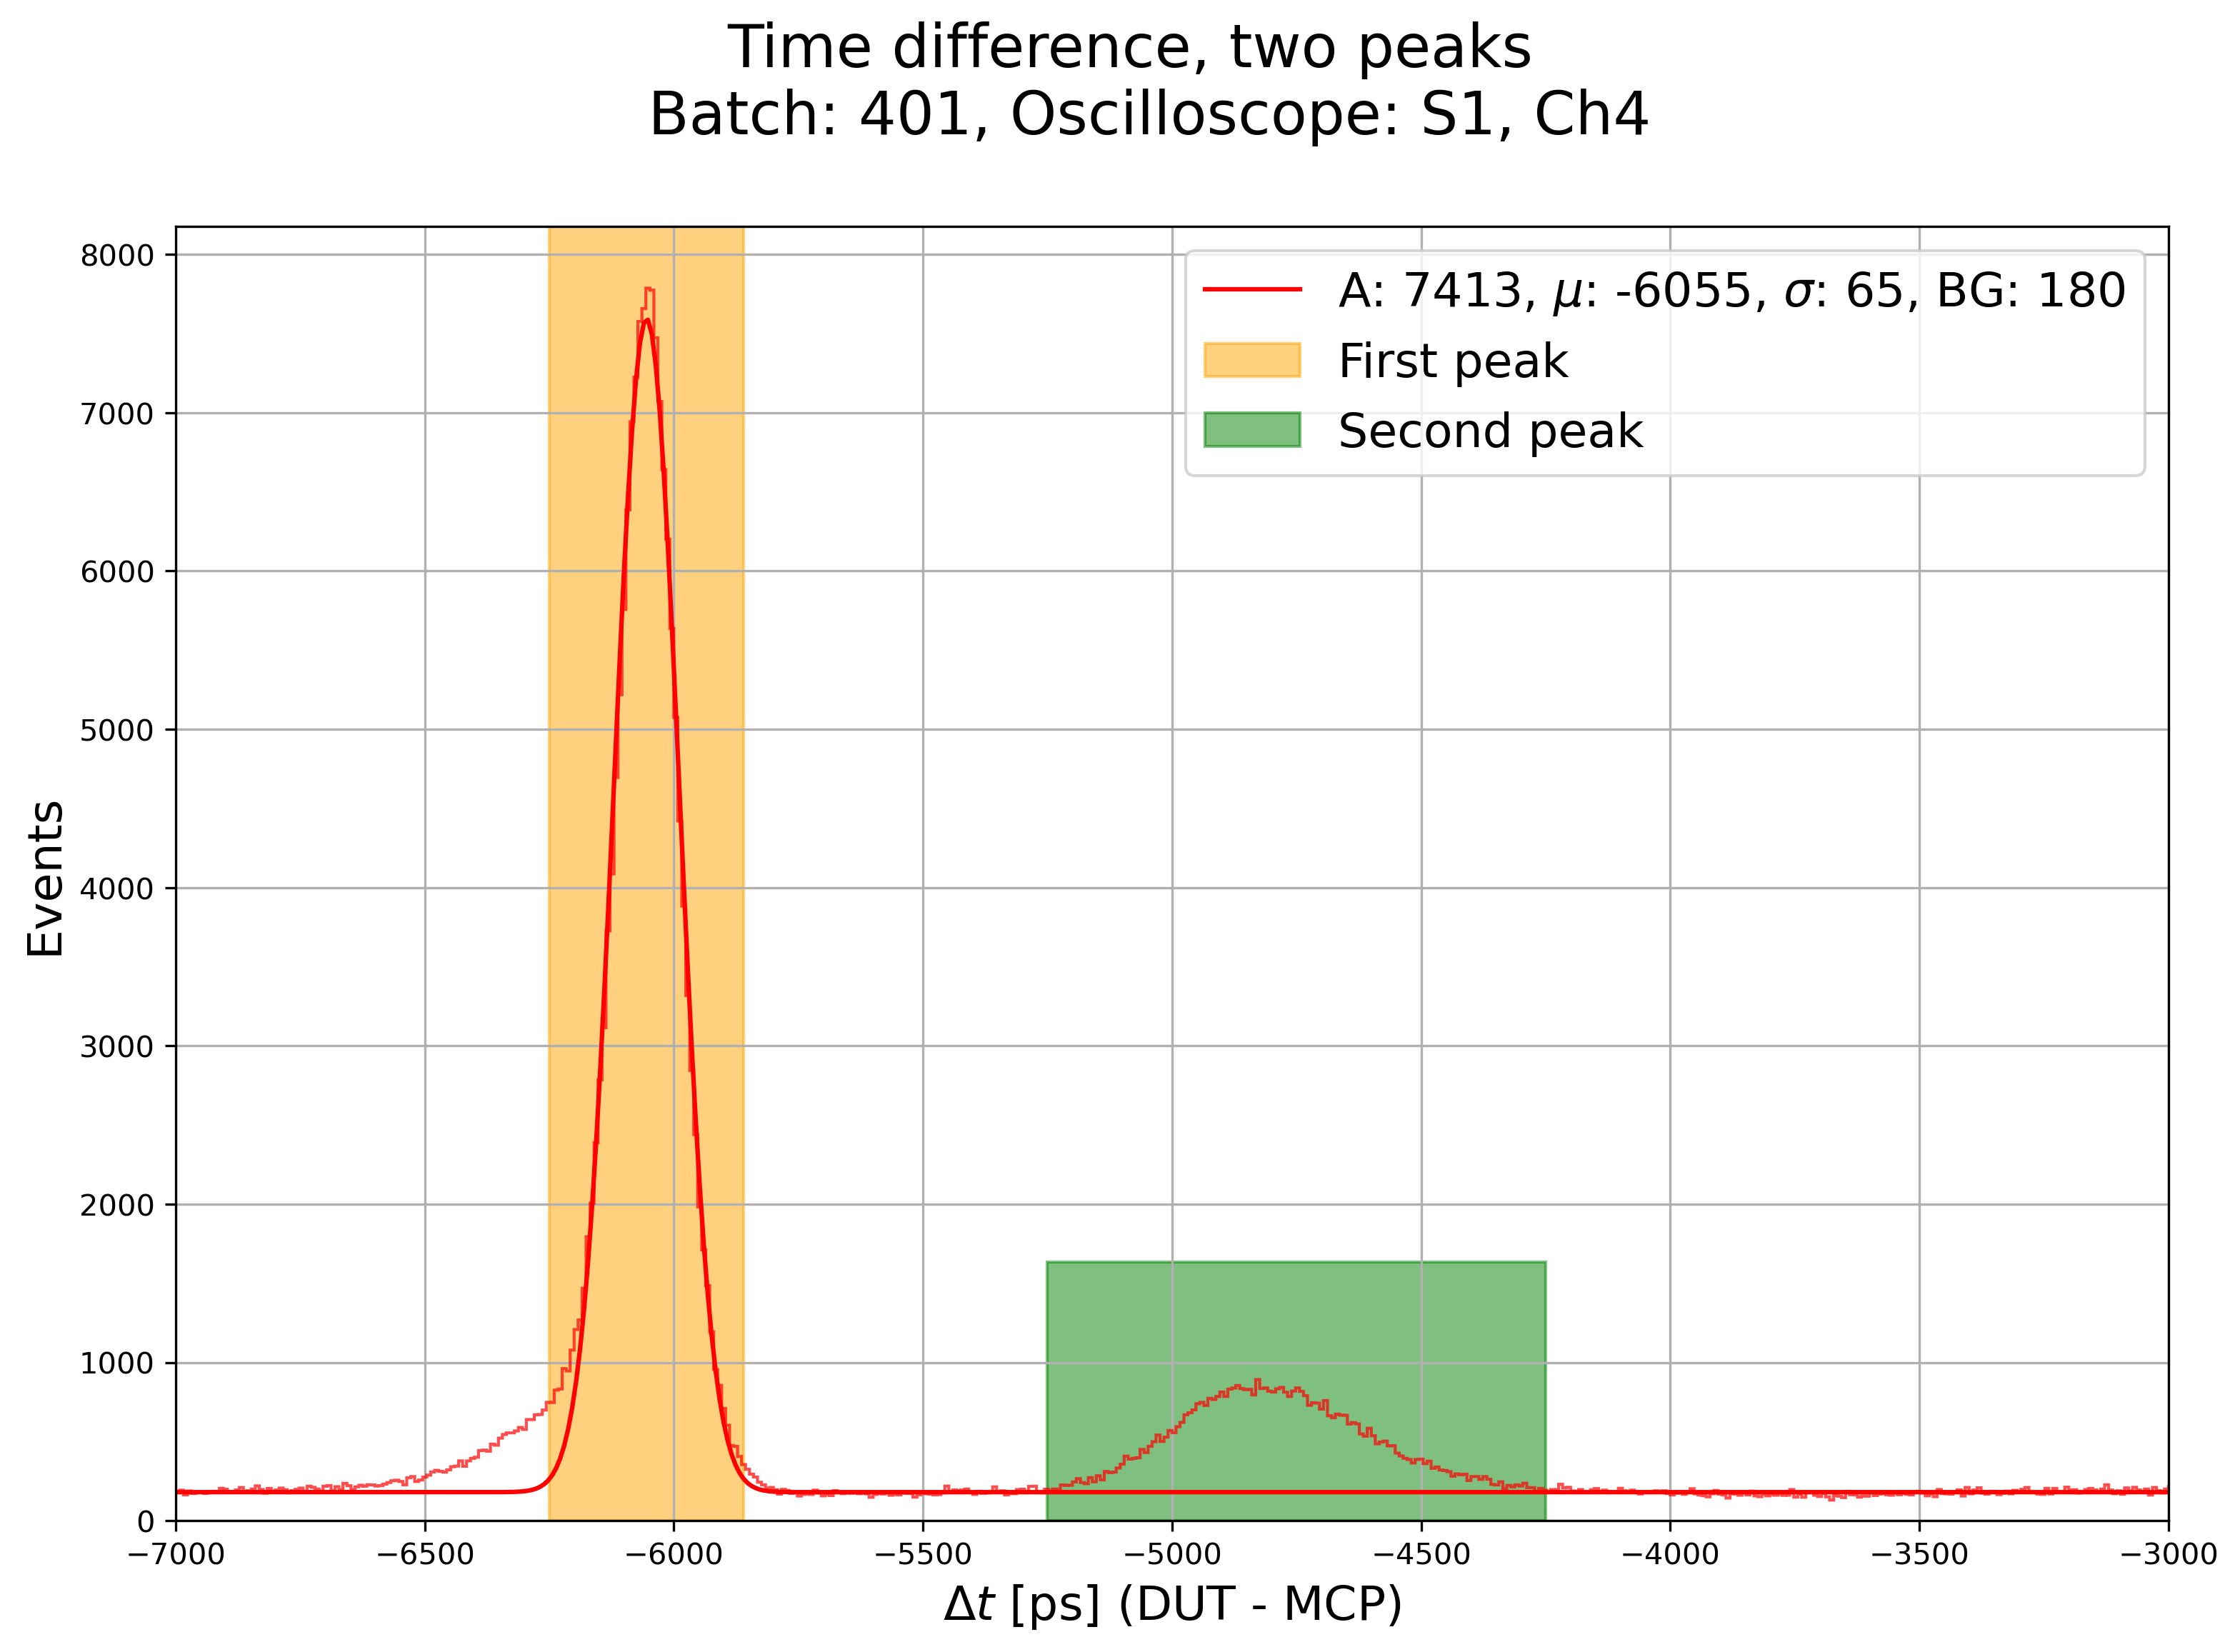
\includegraphics[width=.7\linewidth]{Images/detailed_analysis/time_difference_401_S1_dut_3_with_both_peaks_simple.png}
    \\ [\smallskipamount]
    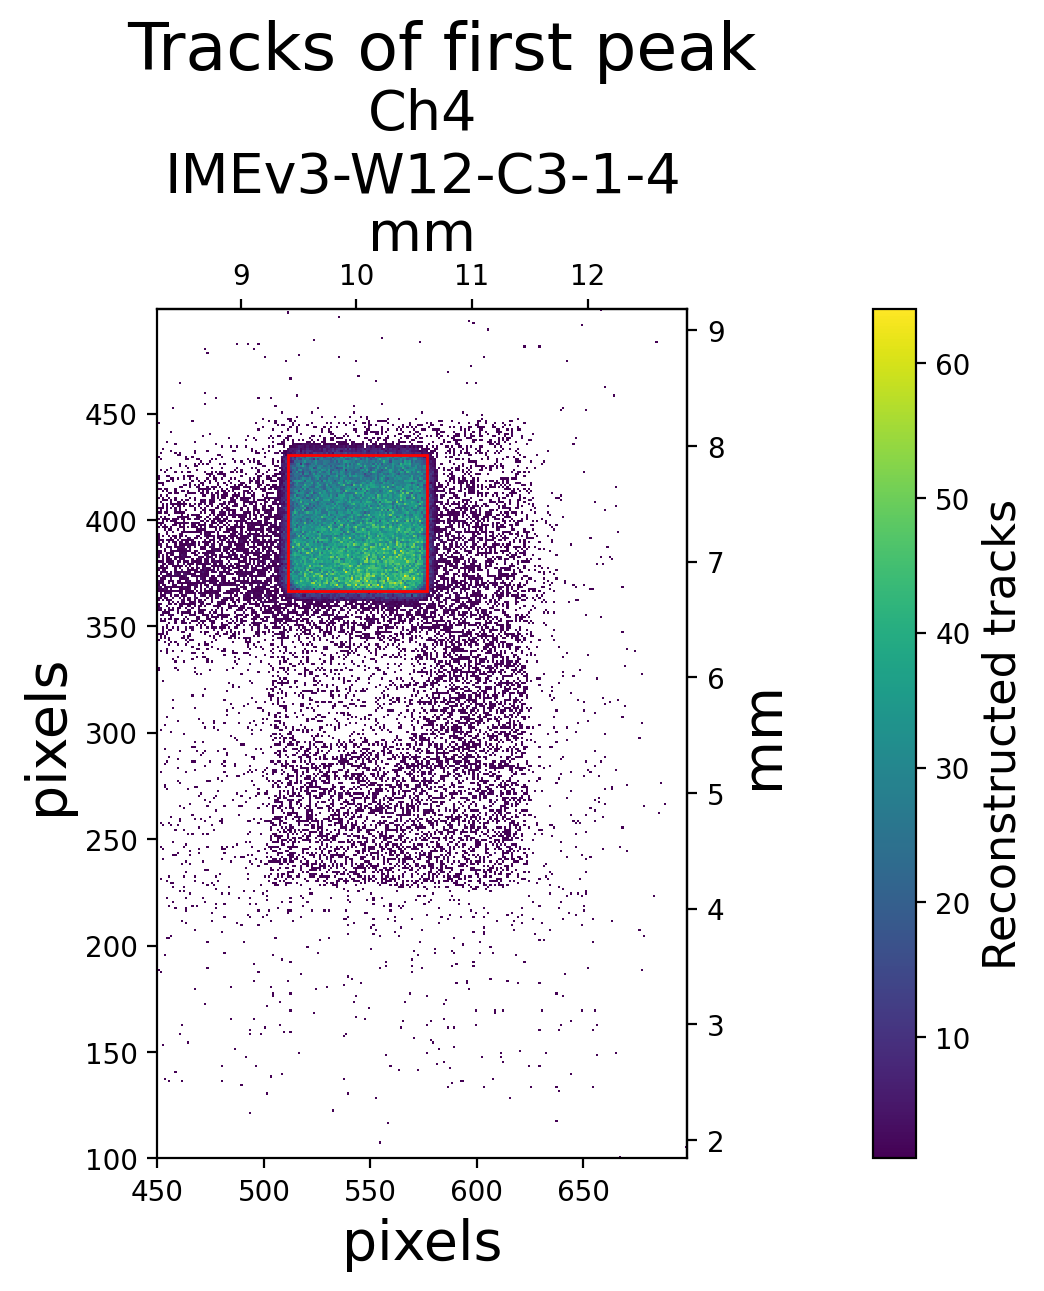
\includegraphics[width=.47\linewidth]{Images/detailed_analysis/2D Tracks 401_S1_dut_3_with_first_peak.png}
    \hfill
    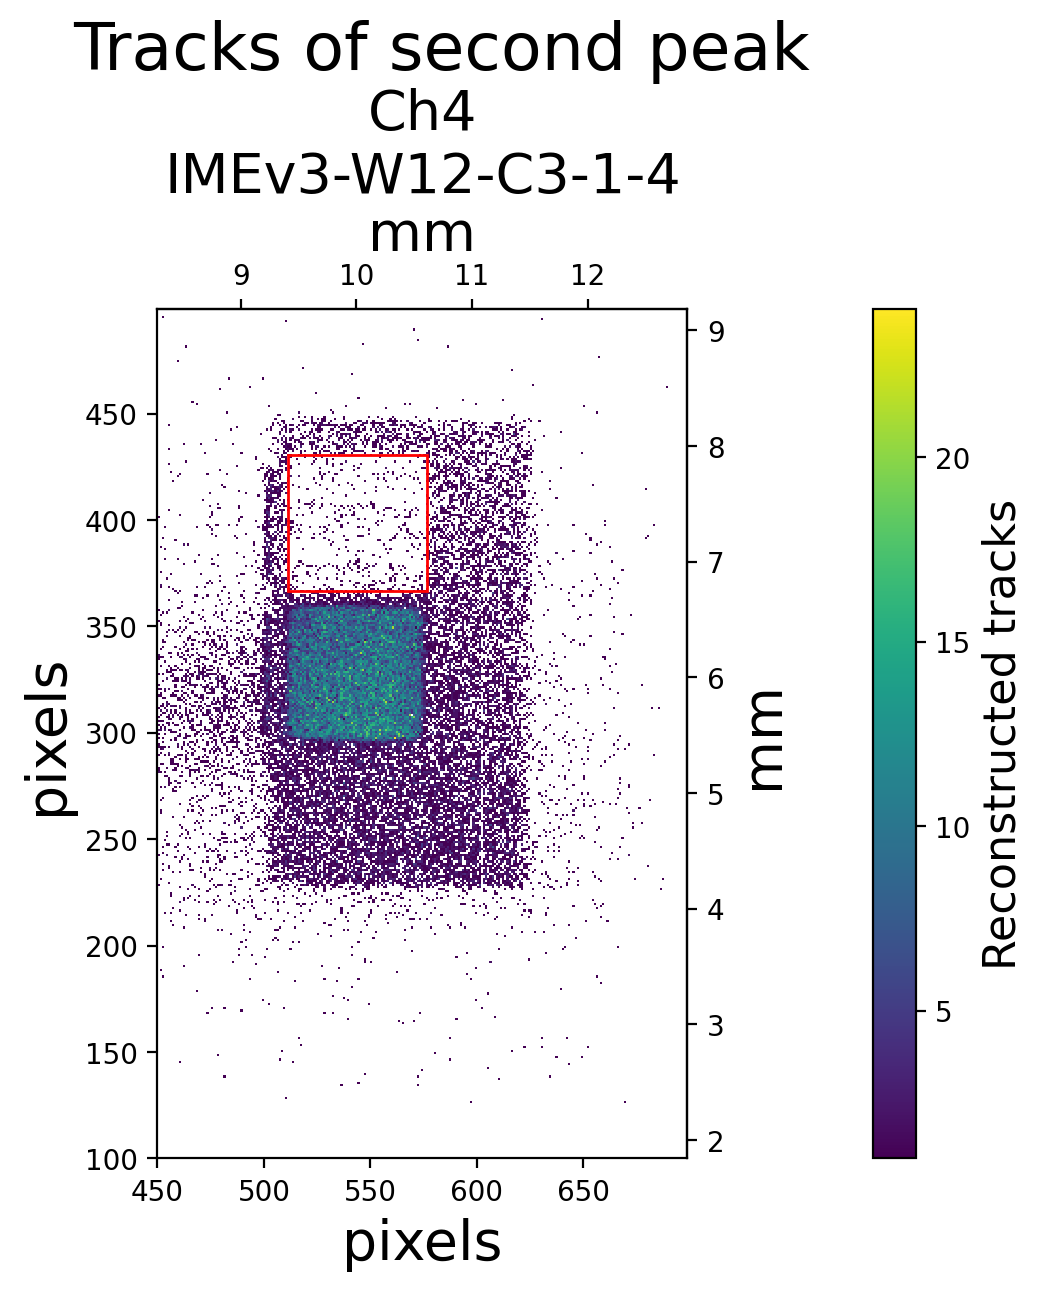
\includegraphics[width=.47\linewidth]{Images/detailed_analysis/2D Tracks 401_S1_dut_3_with_second_peak.png}
    \captionsetup{width=\captionwidth}
    \caption{Top: Time distribution with the first and second peak highlighted in yellow and green, respectively.
    Left: Tracks of events inside yellow interval.
    Right: Tracks of events inside green interval. In red is the outline of the DUT as estimated by the \textit{geometry cut} (\ref{sec:geometry_cut}).}
    \label{fig:time_difference_multiple_peaks_highlight}
\end{figure}
\marginpar{\flushleft Separate the plots so that the text can fit better}


\subsection{Noise from the edges}\label{sec:deviations_from_gaussian}
A secondary effect in the time distribution was the asymmetry between the tails, with the left side notably diverging from a normal distribution. Once again, by singling out only the relevant events, we were able to determine that the ring surrounding the gain layer was responsible for this effect (Figure \ref{fig:time_difference_wide_gaussian}). This further justified our choice of selecting a smaller central area for most of the analysis.

\begin{figure}[h!tbp]
    \centering
    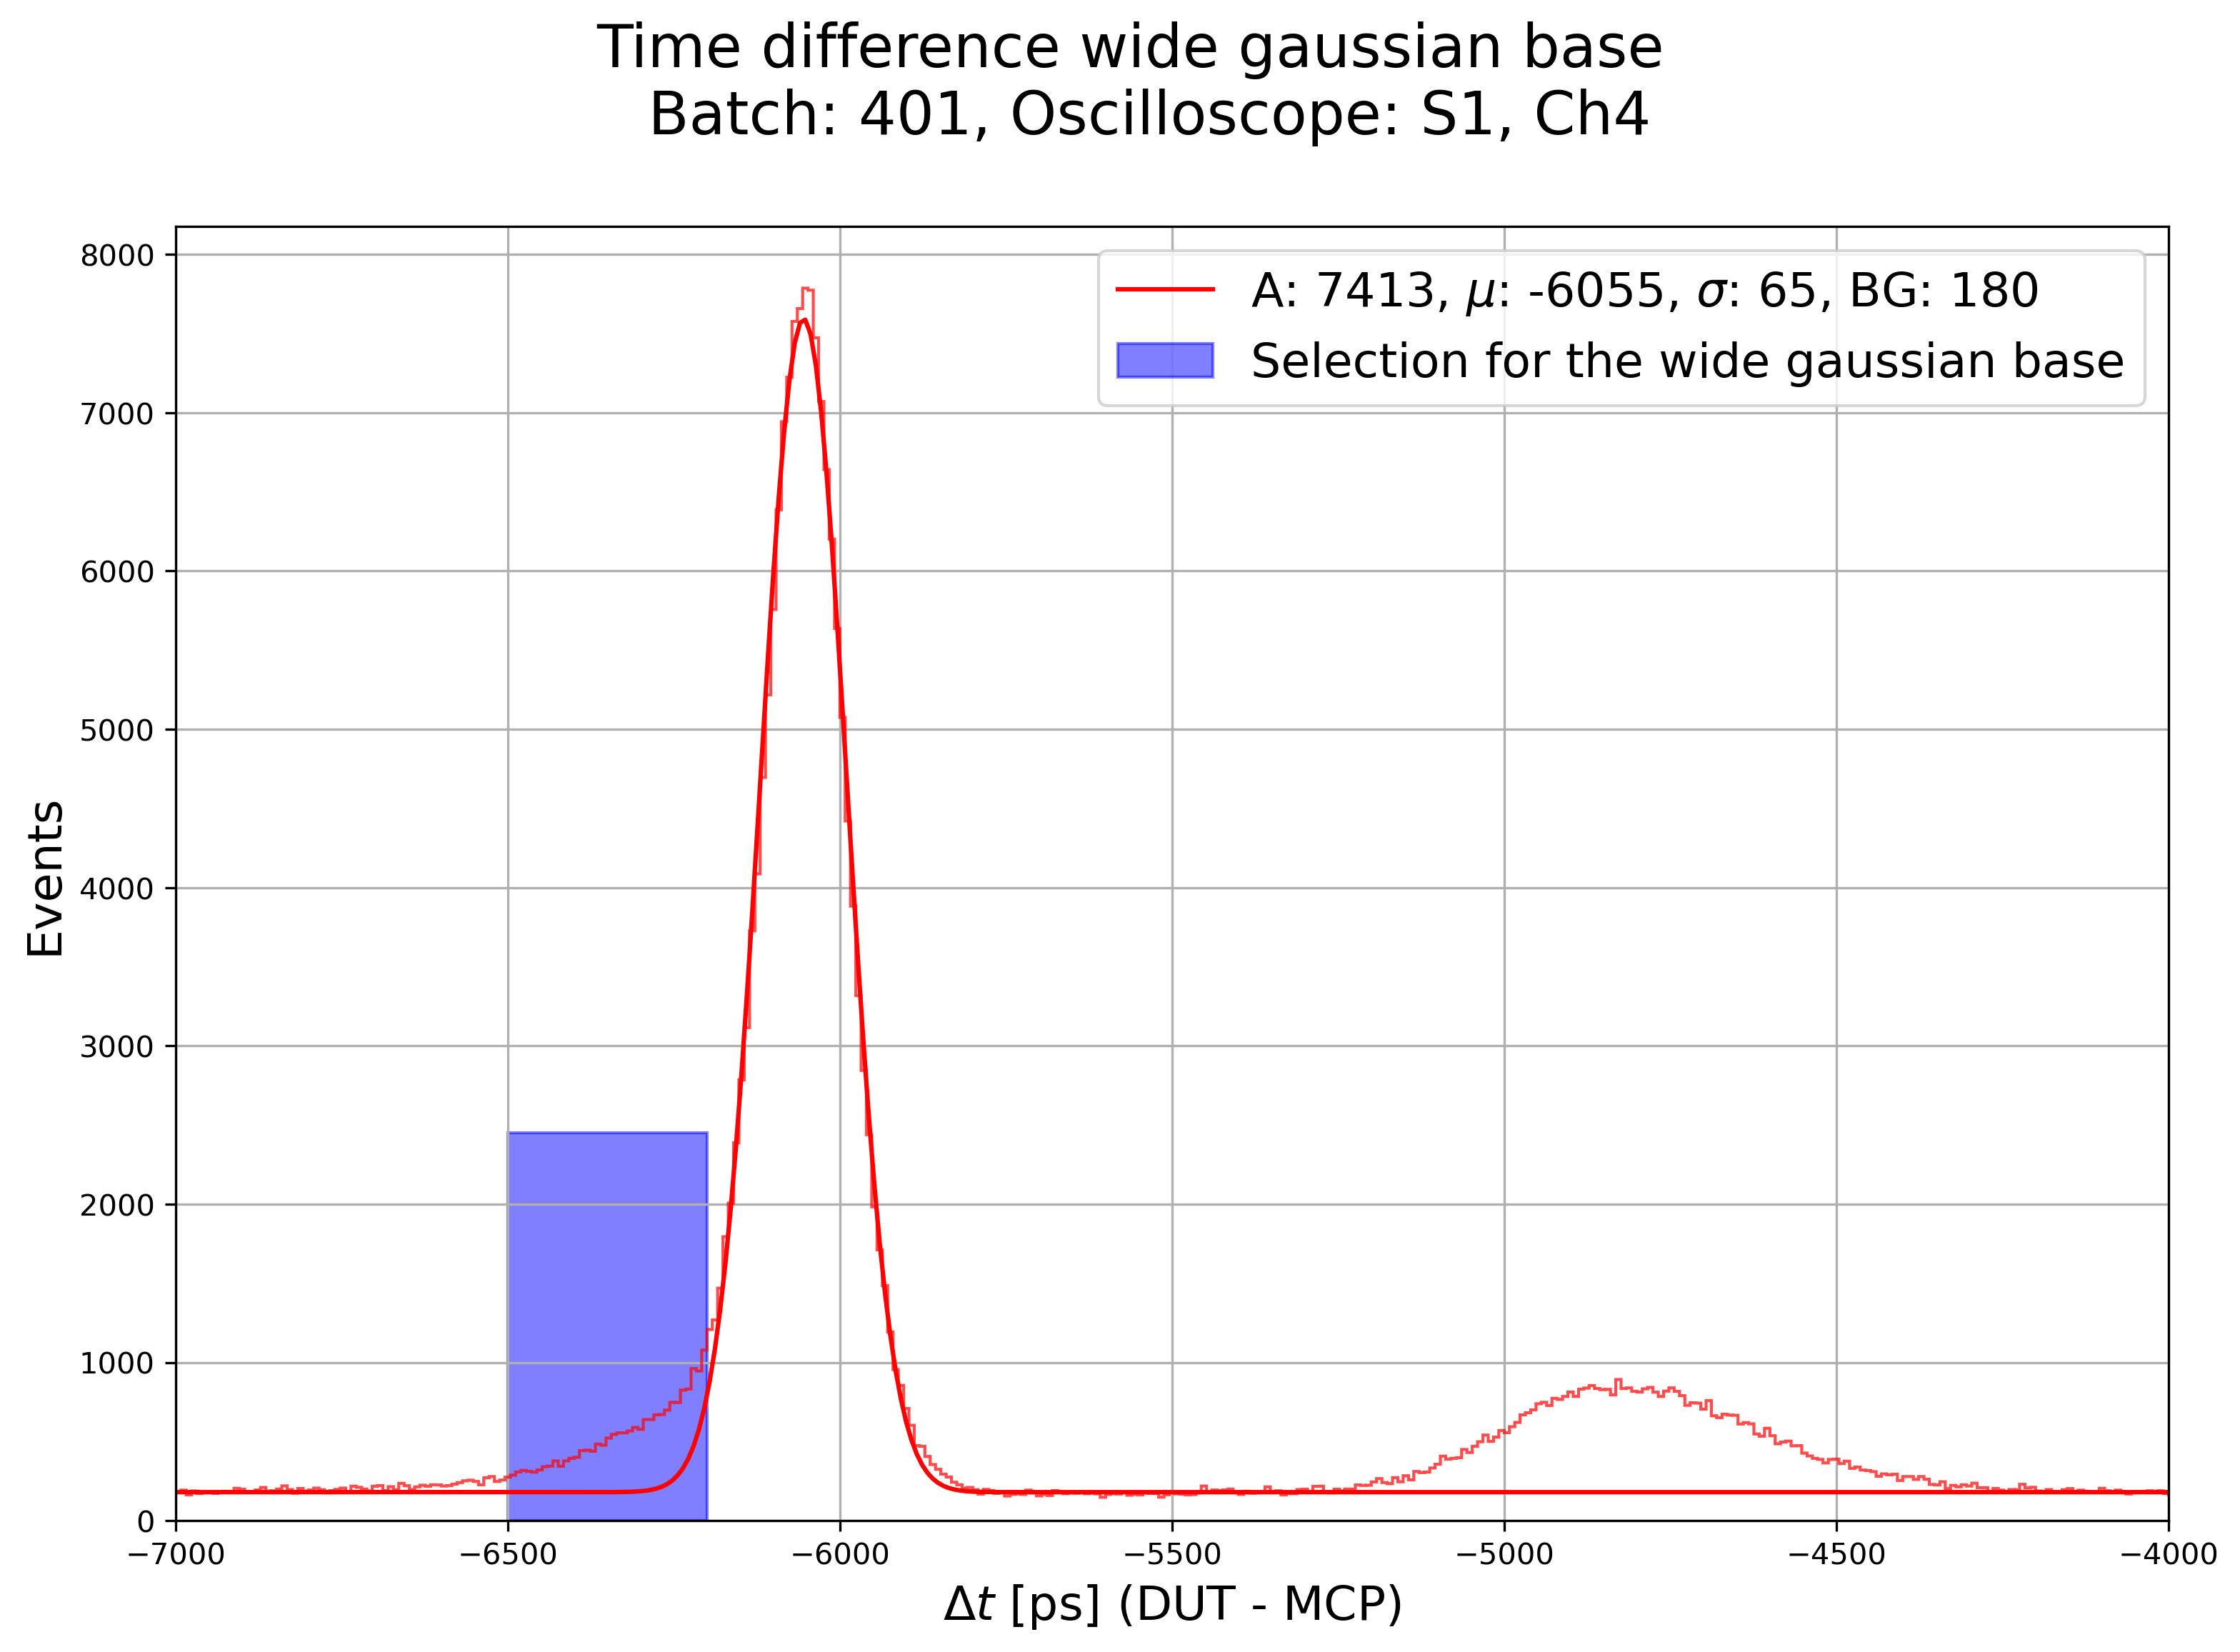
\includegraphics[width=.55\linewidth]{Images/detailed_analysis/time_difference_401_S1_dut_3_with_wide gaussian_left.png}
    \hfill
    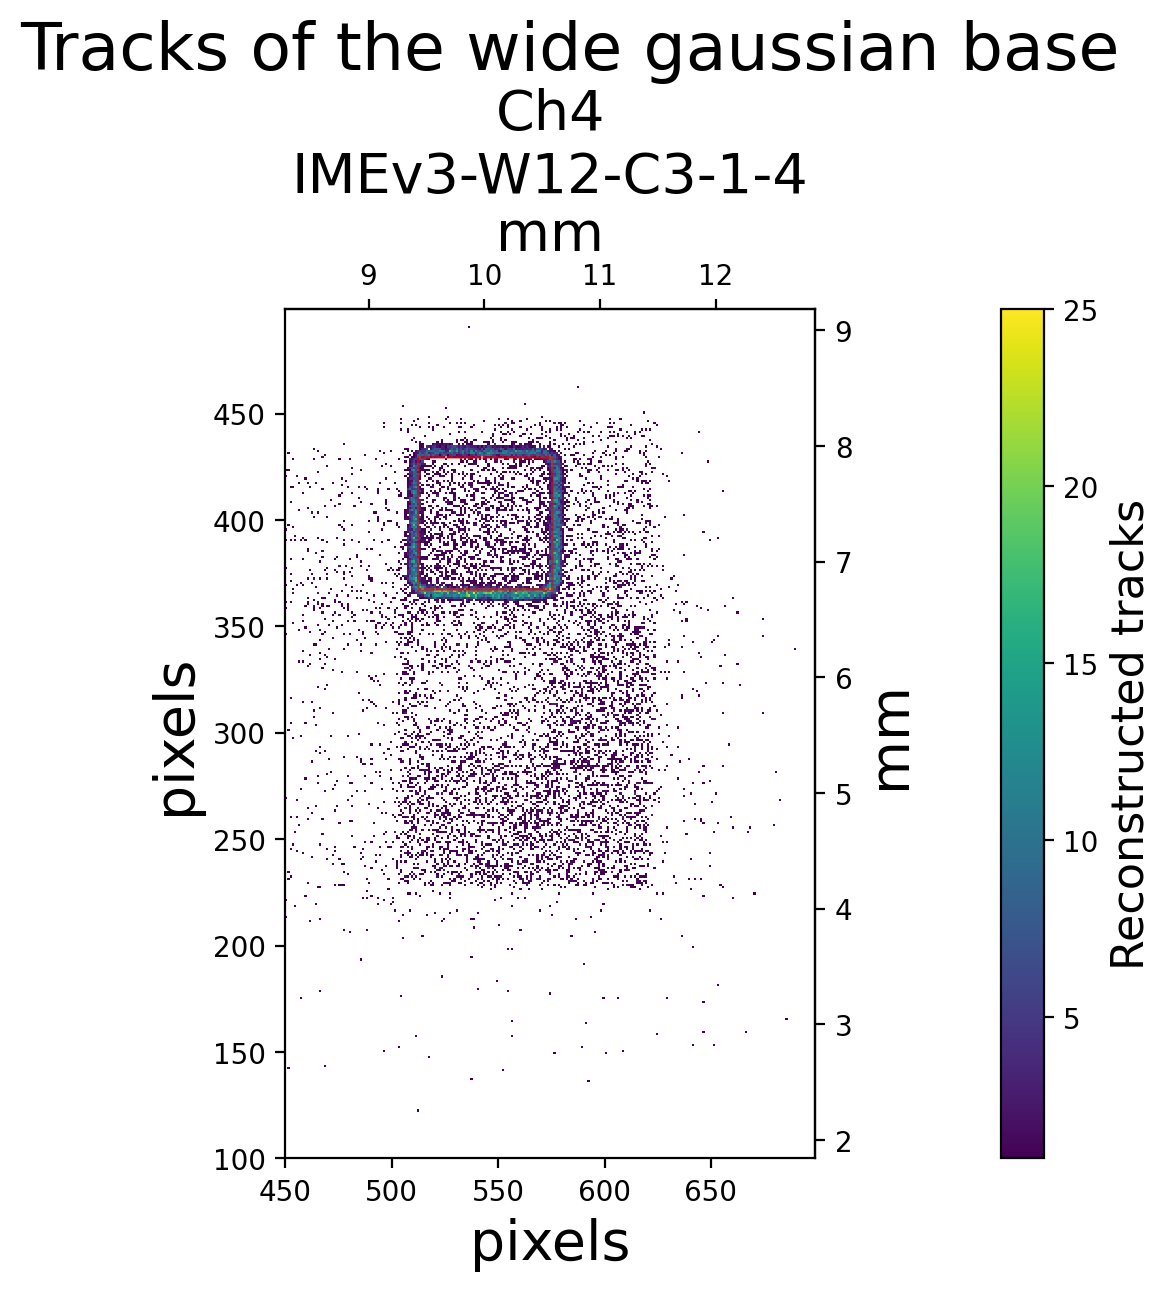
\includegraphics[width=.43\linewidth]{Images/detailed_analysis/2D Tracks 401_S1_dut_3_with_wide_gaussian_base_left.png}
    \captionsetup{width=\captionwidth}
    \caption{Left: selection of the "wide base" of the distribution.
    Right: Tracks of events inside blue interval}
    \label{fig:time_difference_wide_gaussian}
\end{figure}


\subsection{Charge sharing}

\subsection{Interpad study}\label{sec:neighbouring_pads}
\begin{figure}[h!tbp]
    \centering
    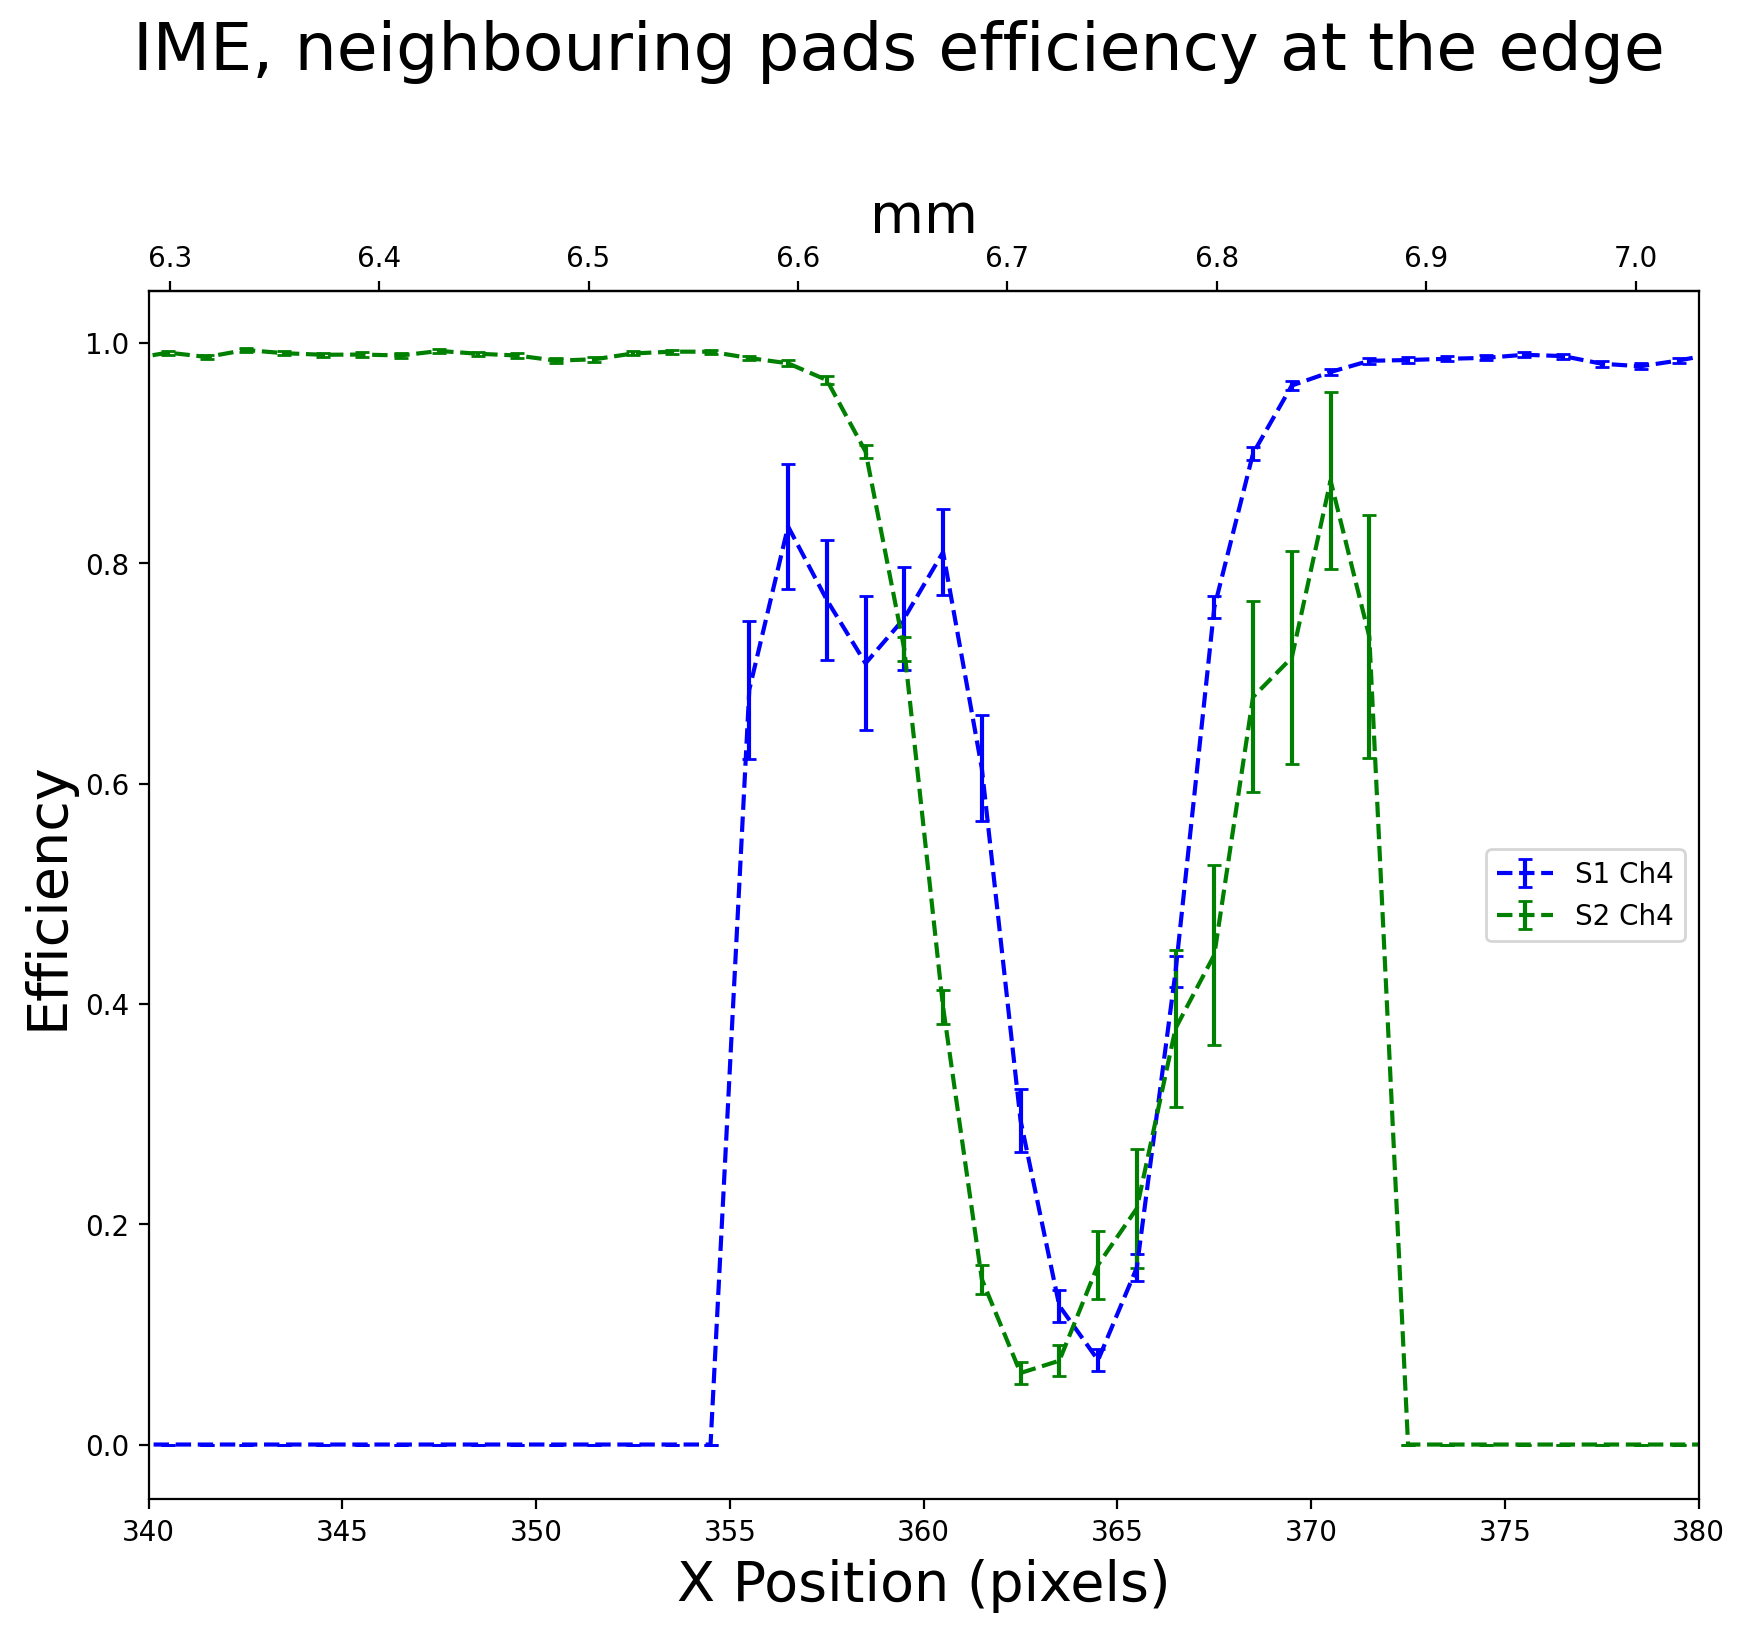
\includegraphics[width=0.5\linewidth]{Images/detailed_analysis/batch 401 duts:3 and 3, edge efficiency studies.png}
    \captionsetup{width=\captionwidth}
    \caption{Caption}
    \label{fig:neighbouring_pads}
\end{figure}

\subsection{Pulse clipping}\label{sec:pulse_clipping}

As briefly mentioned before, there was indirect evidence that the pulses recorded by the oscilloscopes had been "cut" at their highest point. To prove this, the waveforms data was investigated, and a sample is shown in Figure \ref{fig:clipped_pulse}. The outcomes were:

\begin{itemize}
    \item Anomaly in the pulseHeight distribution (Figure \ref{fig:pulseHeight_cut})
    \item irregularities in the charge distribution (Figure \ref{fig:charge_vs_pulseHeight_for_clipping})
\end{itemize}
Fortunately, this effect only impacted a small percentage of the data.

\begin{figure}[h!tbp]
    \centering
    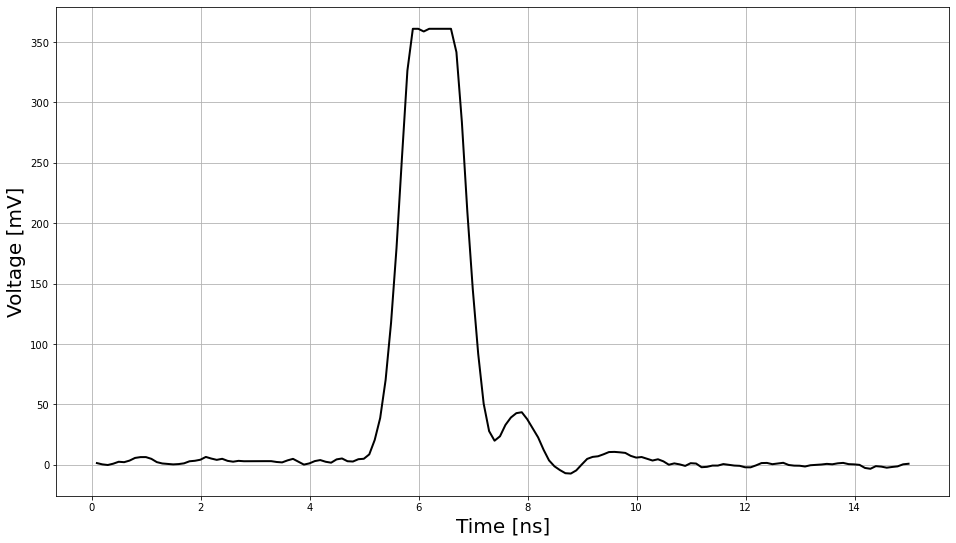
\includegraphics[width=.9\linewidth]{Images/detailed_analysis/Waveform of clipped pulse (ns).png}
    \captionsetup{width=\captionwidth}
    \caption{Example of a single pulse with the highest section cut out}
    \label{fig:clipped_pulse}
\end{figure}
 

\subsubsection{Discrepancies in the tail}\label{subsec:tail_discrepancies}
In a few cases the tail of the distribution deviated considerably from the expected function. We were able to successfully explain this discrepancy with the "clipping" effect in some pulses, due to the limit set to amplitudes registered by the oscilloscopes.
In Section \ref{sec:pulse_clipping} an example of a clipped pulse and its other aftereffects are shown.

In Figure \ref{fig:charge_vs_pulseHeight_for_clipping} (right) the pulseHeight is plotted against the charge and the clipped events appear very clearly at the rightmost part of the plot. This group of events overlapped with the expected charge distribution and could not be removed without modifying it. For this reason, the only solution was to adjust the range of the fit to try to exclude these events.

\begin{figure}[h!tbp]
    \centering
    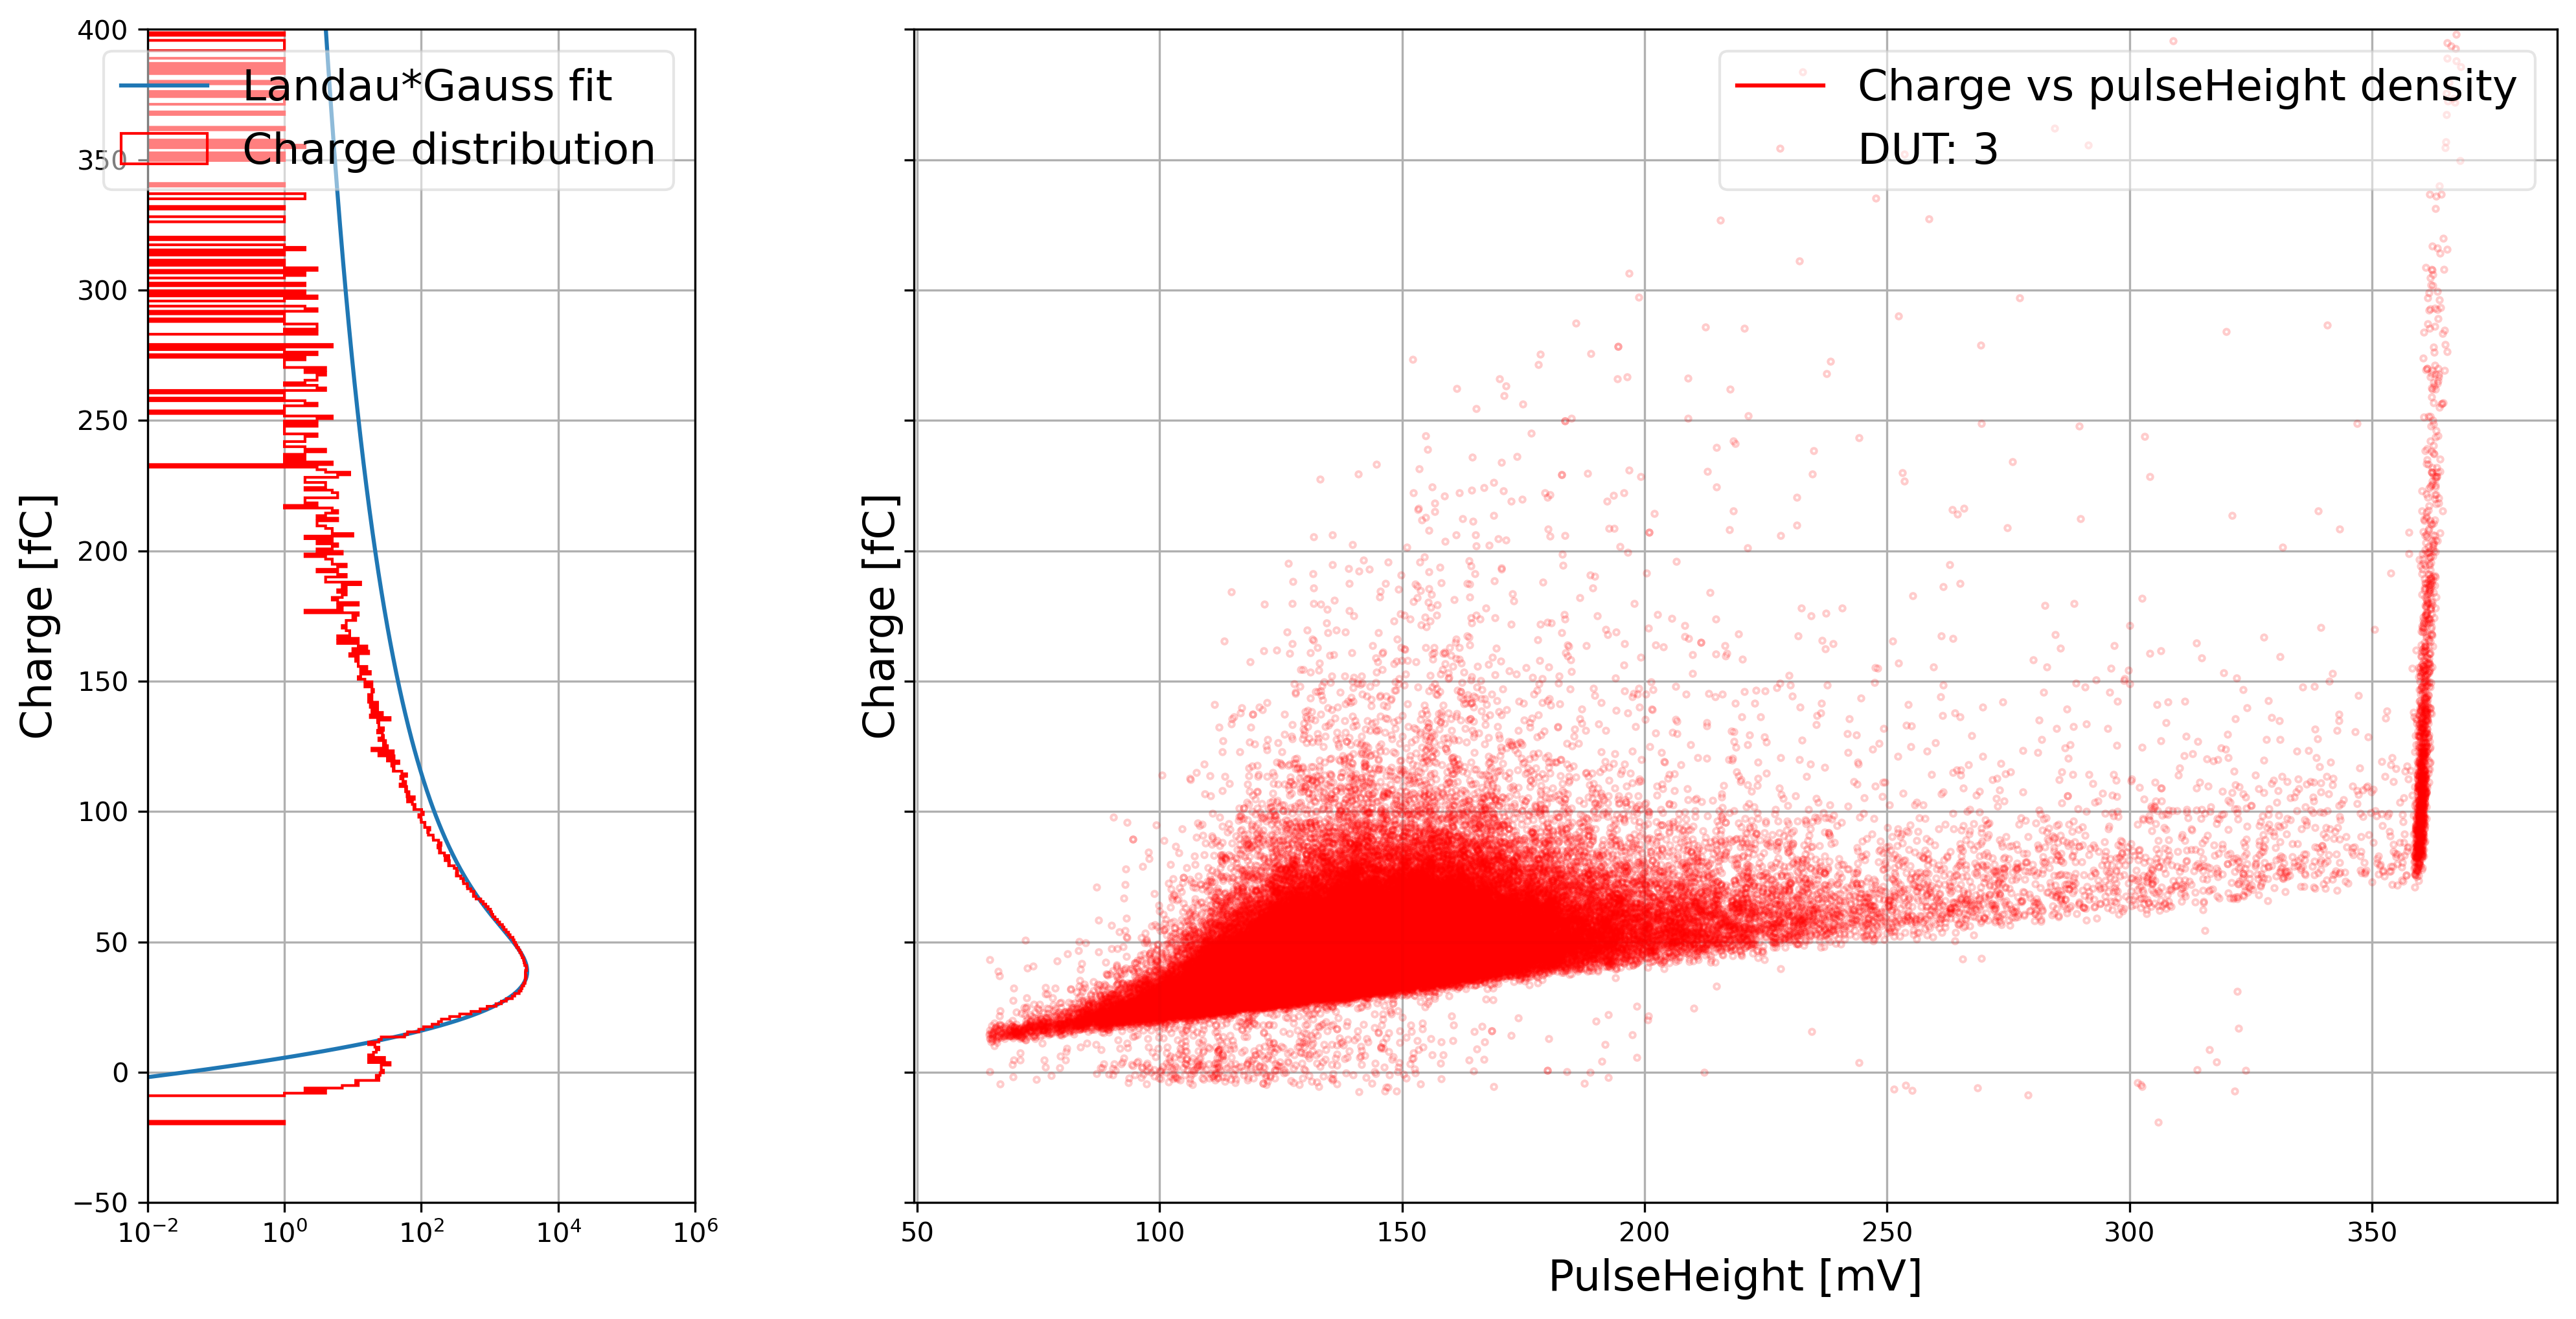
\includegraphics[width=1\linewidth]{Images/charge_plots/Charge_vs_pulseHeight_density_413_S2_dut3.png}
    \captionsetup{width=\captionwidth}
    \caption{Left: distribution of collected charge with Gaussian*Landau fit. Right: scatter plot PulseHeight vs Charge, revealing the cause of the irregular tail}
    \label{fig:charge_vs_pulseHeight_for_clipping}
\end{figure}


\subsection{Temperature fluctuations}\label{sec:temperature_fluctuations}


% \subsection{Charge sharing}\label{sec:charge_sharing}


